\documentclass[en]{../../../../../../eplexam}

\usepackage{../../../../../../eplunits}
\usepackage{../../../../../../eplcode}

\hypertitle{Programming Languages Concepts}{6}{INGI}{1131}{2011}{Janvier}{Majeure}
{Legat Beno\^it}
{Peter Van Roy}

\lstset{language={Oz},morekeywords={for,do,lazy}}

\paragraph{Useful resource}
\url{http://www.forum-epl.be/viewtopic.php?t=7809}.

\section{An oscillator with a delay gate and a xor gate}
\begin{center}
  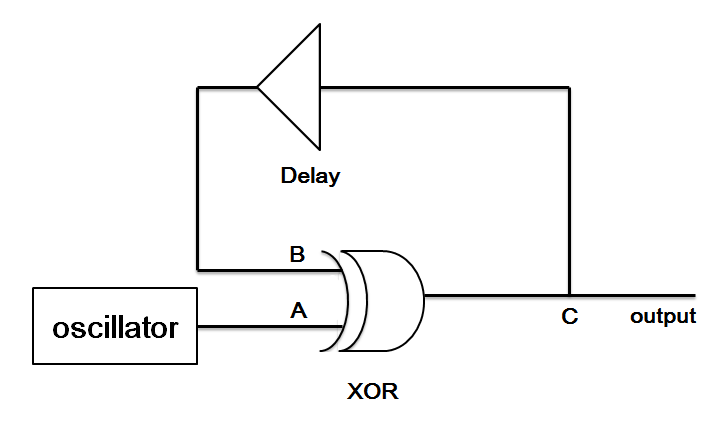
\includegraphics[width=0.6\textwidth]{circuit.png}
\end{center}
\begin{itemize}
  \item Implement each element using the simulation technique
    used in the course.
    All the elements are lazy.
  \item Give the code for the circuit shown in the figure.
  \item Show the first and second output of this circuit.
  \item Prove rigorously that the output is alternating with
    \lstinline|1| and \lstinline|0|.
    Represent the streams symbolically, for example
    A = $a_0$|$a_1$|$\cdots$,
    and analogously for B and C.
  \item Explain the lazy activations and lazy suspensions.
\end{itemize}

\section{A semi-infinite helix}
Semi-hélice infinie
\begin{enumerate}
  \item Un agent \lstinline|I| lié à \lstinline|i+1|, \lstinline|i-1|, \lstinline|i+10|, \lstinline|i-10| en Active Object ou Port Object reçoit
    \begin{lstlisting}
set(I A)
get(I X)
    \end{lstlisting}
    avec \lstinline|A| et \lstinline|X| des State et \lstinline|set| et \lstinline|get| : deux cas : soit \lstinline|I| correspond avec celui de l'objet sur lequel le message est balancé, et donc l'opération set règle l'état à \lstinline|A| et la get bind \lstinline|X| à l'état de l'objet, ou bien le message est renvoyé sur un objet dont le \lstinline|I| est le plus proche.

    Chaque objet connait le suivant et le précédent, ainsi que le dixième après lui, et le dixième avant lui. Un peu comme une structure chainée, mais avec des raccourcis de 10 éléments qui sont utilisés quand c’est plus logique que de rebalancer ça chez le voisin direct.
  \item Créer une fonction \lstinline|{MakeAgent I}| qui retourne un active object ou un port object qui porte le numéro \lstinline|I|.
  \item Implémenter \lstinline|{BuildHelix}| which build the helix using lazy paradigm.
    It returns a list of agents.
\end{enumerate}

\begin{solution}
  \lstinputlisting{q2.oz}
\end{solution}

\section{Building a transaction protocol}
\begin{enumerate}
  \item Pourquoi reentrant lock + exemple d’abstractions qui les nécessitent?
  \item Pourquoi reentrant lock pas suffisants pour shared date structures + exemple abstractions qui les nécessitent? + définition de monitor + opérations + sémantique via JAVA.
  \item Pourquoi reentrant lock pas suffisants pour update dans Data-Base (plusieurs raisons) + définition de transactions + en quoi celles-ci sont-elles des solutions aux problèmes.
  \item Pourquoi deadlock problem dans transactions: exemple 2 transactions en deadlocks.
    Comment manager gère-t-il ces deadlocks ?  + définition deadlock + ``Wait-for'' graph.
\end{enumerate}

\end{document}
